\documentclass{article}

\usepackage[spanish]{babel}
\usepackage[utf8]{inputenc}
\usepackage[right=1.5cm,left=1.5cm,top=1.5cm,bottom=1.5cm]{geometry}

\title{Taller 3A\\ Estadística genómica}
\author{Juan David Henao Sánchez}

\usepackage{Sweave}
\begin{document}
\Sconcordance{concordance:JuanHenao_Taller3A.tex:JuanHenao_Taller3A.Rnw:%
1 9 1 1 0 9 1 1 2 1 0 1 1 3 0 2 2 1 0 1 1 5 0 1 1 19 0 2 2 5 0 2 2 1 0 %
2 1 11 0 2 1 3 0 2 2 1 0 1 1 7 0 2 2 20 0 2 2 1 0 2 1 19 0 2 2 5 0 2 2 %
1 0 1 1 5 0 1 1 11 0 1 2 2 1}


\maketitle

\section*{Sobre unos datos del GEO (una sola medición en el tiempo) que comparen dos condiciones, identifique los genes diferencialmente expresados usando acde:
}

\begin{Schunk}
\begin{Sinput}
> library(acde)
> library("DESeq")
> #########################
> data <- read.table("GSE58972_RELA_6h_processed_data.txt", h=T)
> dim(data)
\end{Sinput}
\begin{Soutput}
[1] 23284     8
\end{Soutput}
\begin{Sinput}
> head(data)
\end{Sinput}
\begin{Soutput}
           gene description WT_6h_1 WT_6h_2 WT_6h_3 RELA_6h_1 RELA_6h_2
1 0610005C13Rik          na       9      12      12        11        16
2 0610007C21Rik          na     534     581     562       512       537
3 0610007L01Rik          na    2124    2197    2168      2811      2706
4 0610007N19Rik          na      17      26      21        18        20
5 0610007P08Rik          na    1410    1504    1543      1546      1577
6 0610007P14Rik          na    2049    2008    2074      2192      2192
  RELA_6h_3
1        10
2       501
3      2265
4        15
5      1353
6      1968
\end{Soutput}
\end{Schunk}
\begin{Schunk}
\begin{Sinput}
> boxplot(data[, 3:8], main="Boxplot Mus musculus", col="lightgreen", cex.names=0.2, las=2)
\end{Sinput}
\end{Schunk}
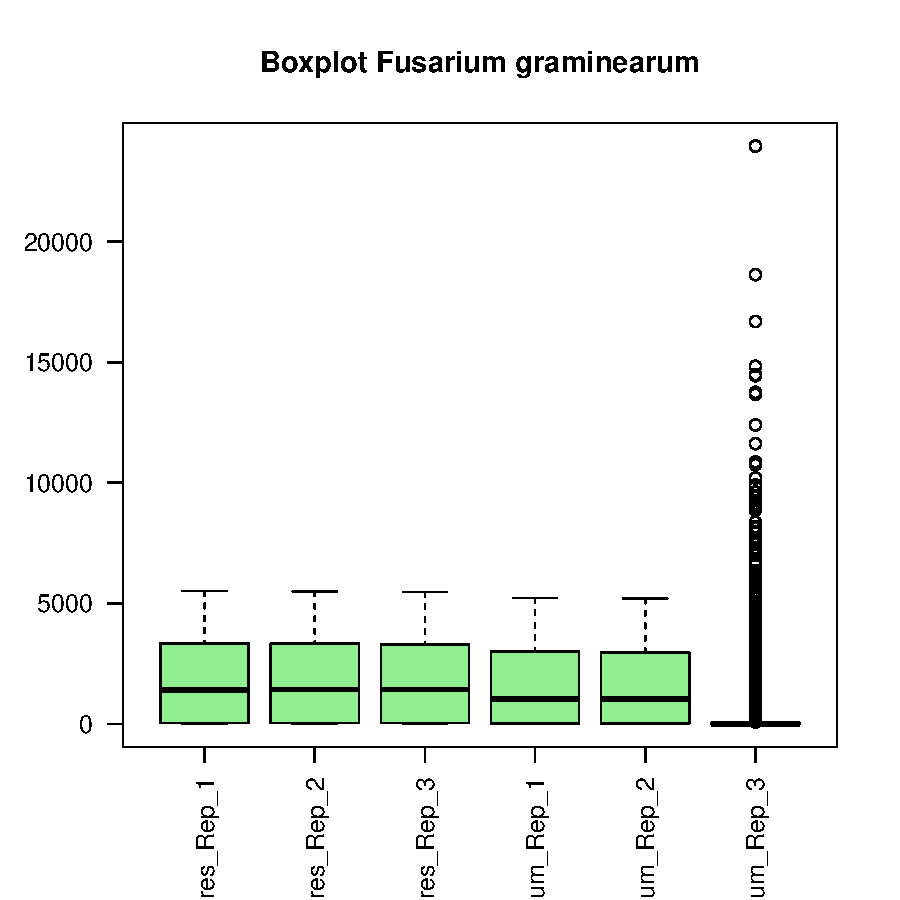
\includegraphics{JuanHenao_Taller3A-002}
\begin{Schunk}
\begin{Sinput}
> rownames(data) <- data$gene
> countsTable <- data[,3:8]
> head(countsTable)
\end{Sinput}
\begin{Soutput}
              WT_6h_1 WT_6h_2 WT_6h_3 RELA_6h_1 RELA_6h_2 RELA_6h_3
0610005C13Rik       9      12      12        11        16        10
0610007C21Rik     534     581     562       512       537       501
0610007L01Rik    2124    2197    2168      2811      2706      2265
0610007N19Rik      17      26      21        18        20        15
0610007P08Rik    1410    1504    1543      1546      1577      1353
0610007P14Rik    2049    2008    2074      2192      2192      1968
\end{Soutput}
\begin{Sinput}
> conds <- factor( c( "S1", "S2", "S3", "M1","M2","M3"))
> newcds <- newCountDataSet( countsTable, conds )
\end{Sinput}
\end{Schunk}

\end{document}
